



%%%%%%%%%%%%%%%%%%%%%%%%%%%%%%%%%%%%%%%%%%%%%%%%%%%%%%%%%%%%
\clearpage
\appendix
\section{Appendix}
%%%%%%%%%%%%%%%%%%%%%%%%%%%%%%%%%%%%%%%%%%%%%%%%%%%%%%%%%%%%


%%%%%%%%%%%%%%%%%%%%%%%%%%%%%%%%%%%%%%%%%%%%%%%%%%%%%%%%%%%%
\subsection{Two-dimensional likelihood}
\label{sec:appendix_2d}
%%%%%%%%%%%%%%%%%%%%%%%%%%%%%%%%%%%%%%%%%%%%%%%%%%%%%%%%%%%%

Instead of estimating the density over the full 15-dimensional
phase-space, we also check some of the approaches on the much simpler
problem of estimating the density of the two-dimensional distribution
$p(p_{T,j1}, \Delta \phi_{jj} ; \boldtheta)$.




%%%%%%%%%%%%%%%%%%%%%%%%%%%%%%%%%%%%%%%%%%%%%%%%%%%%%%%%%%%%
\subsubsection{Benchmark hypothesis test}
%%%%%%%%%%%%%%%%%%%%%%%%%%%%%%%%%%%%%%%%%%%%%%%%%%%%%%%%%%%%

For two benchmark parameter points
%
\begin{equation}
  \boldtheta_0 = \twovec{-0.2} {-0.2} \,, \quad
  \boldtheta_1 = \twovec{0.2} {0.2}
  \label{eq:pointwise_tuning_benchmarks}
\end{equation}
%
we first analyse how well \toolfont{carl} can estimate the likelihood ratio
%
\begin{equation}
  r(\boldx) = \frac {p(\boldx | \boldtheta_0)}  {p(\boldx | \boldtheta_1)}
  \label{eq:pointwise_tuning_r}
\end{equation}
%
depending on the classifier, its hyperparameters, and a number of
different settings.

For each of the four feature sets outlined above (2D, medium set, full
kinematics, full kinematics plus derived variables), we tune the
parameters in two steps. First, we perform a randomized scan over
the hyperparameters, maximizing the classification power between event
samples sampled from $p(\boldx | \boldtheta_0)$ and
$p(\boldx | \boldtheta_1)$. In a second step we finetune these
parameters on the mean squared error between the \toolfont{carl}
estimate $\log \hat{r}(\boldx)$ and the true value $\log r(\boldx)$.

The first classifier we consider is a \emph{random forest}, more
precisely extremely randomized trees, in the
\toolfont{sklearn.ensemble.ExtraTreesClassifier} implementation. The
following parameters are tuned:
%
\begin{itemize}
  \item \toolfont{n\_estimators}, the number of trees in the forest;
  \item \toolfont{max\_features}, the number of features considered in
    the search for the best split;
  \item \toolfont{max\_depth}, the maximum depth of the trees;
  \item \toolfont{min\_samples\_split}, the minimum fraction of events
    at a node required for a split; and
  \item \toolfont{min\_samples\_leaf}, the minimum fraction of events
    in a leaf.
\end{itemize}

A \emph{multi-layer perceptron} implemented as a
\toolfont{sklearn.neural\_network.MLPClassifier} is our second
classifier. We optimize the following parameters:
%
\begin{itemize}
  \item \toolfont{hidden\_layer\_sizes}, describing the number of hidden
  layers and the number of neurons in each layer;
  \item \toolfont{activation}, the activation function; and
  \item \toolfont{alpha}, an $L^2$ penalty term.
\end{itemize}

For both classifiers, the kinematic features are first rescaled to a
normal distribution with a
\toolfont{sklearn.preprocessing.StandardScaler}.



\begin{figure}
  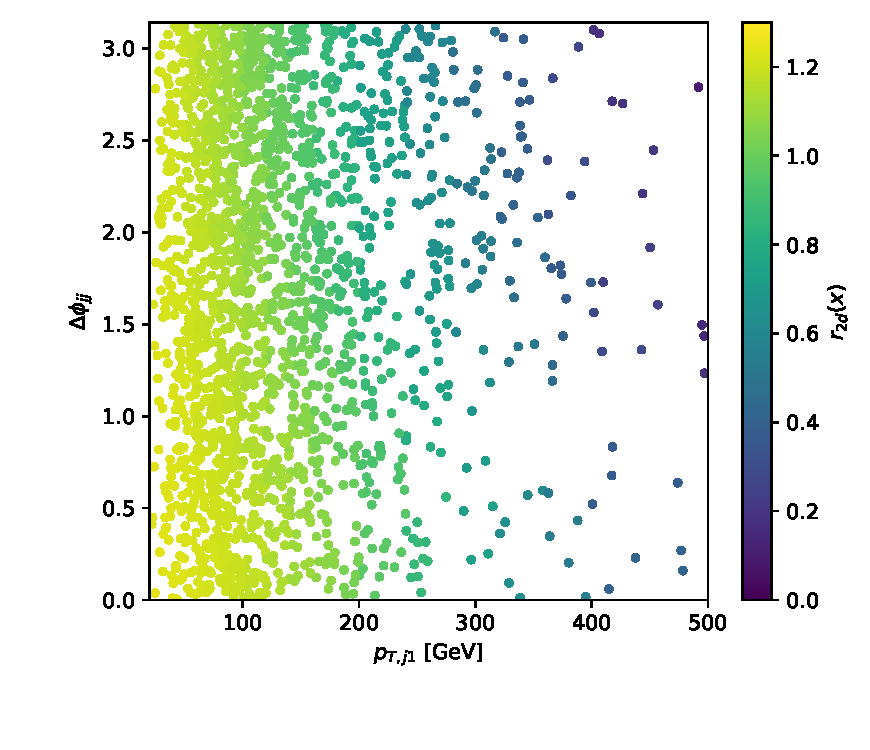
\includegraphics[height=0.45\textwidth]{figures/pointwise_tuning_2d/r_over_x.pdf}
  \caption{Truth likelihood ratio $r(\boldx)$ as defined in
    \autoref{eq:pointwise_tuning_r} for the 2D case. The effect of the
    binning in the calculation of $r_{\text{2d}}(\boldx)$ is clearly
    visible.}
  \label{fig:pointwise_tuning_2d_r_x}
\end{figure}

First we only consider two kinematic features, the leading jet
momentum and the azimuthal angle between the two
jets. \autoref{fig:pointwise_tuning_2d_r_x} shows how the truth
likelihood ratio between the two points defined in
\autoref{eq:pointwise_tuning_benchmarks} depends on these observables.

\begin{table}
\begin{tabular}{ll rrr}
  \toprule 
  Classifier & Parameter & Range & Good & Best \\
  \midrule
  Random forest & \toolfont{n\_estimators} & $50 \dots 200$ & $50 \dots 200$  & $100$ \\
  & \toolfont{max\_features} & $1, 2$ & $2$ & $2$ \\
  & \toolfont{max\_depth} & $1 \dots 20, \infty$ & $6\dots 8$ & $8$ \\
  & \toolfont{min\_samples\_split} & $0 \dots 1$ & $10^{-4} \dots 10^{-3}$ & $10^{-3}$ \\
  & \toolfont{min\_samples\_leaf} & $0 \dots 0.5$ & $0$ & $0$ \\
  \midrule
  Neural network & number of hidden layers & $1,2,3$ & $2$ & $2$\\
  & neurons at each layer & $2\dots 20$ per layer & $(20,20)$ & $(20,20)$\\
  & activation function & $\tanh, \relu, \logistic$ & $\tanh, \relu$ & $\tanh$ \\
  & $\alpha$ & $0\dots 100$ & $0\dots 1$ & $10^{-3}$\\
  \bottomrule
\end{tabular}
\caption{Hyperparameter scan on the classification problem between
  $\boldtheta_0$ and $\boldtheta_1$ for the 2D case. For both classifier
  and each parameter we show the considered range, the range of values
  with good results (\ie ROC AUC close to the optimum),
  and the (rounded) optimal value. }
 \label{tbl:pointwise_tuning_2d_parameters}
\end{table}

We first tune hyperparameters with a randomized scan on the
classification problem between unweighted event samples drawn from
$p(\boldx | \boldtheta_0)$ and $p(\boldx | \boldtheta_1)$. Using
\toolfont{sklearn.model\_selection.RandomizedSearchCV}, we optimize on
the ROC AUC. We give the optimal parameters in
\autoref{tbl:pointwise_tuning_2d_parameters}. Key to a good
performance for the random forest is a maximal depth around 8. Only
considering one feature at each splitting or requiring a large number
of events for a splitting or at each leaf lead to a worse
performance. Above a certain threshold, the number of trees does not
have a huge effect. For the neural network, two hidden layers with 20
neurons each and tanh or ReLU activation functions perform best, while
the value of the regulator $\alpha$ is not very important.

\begin{figure}
  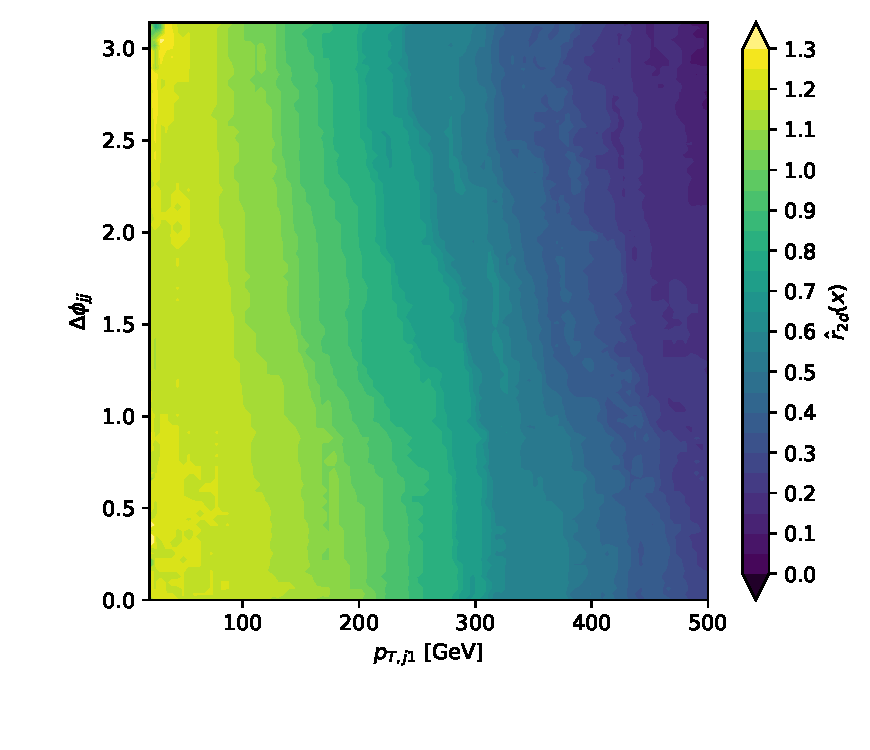
\includegraphics[height=0.45\textwidth]{figures/pointwise_tuning_2d/rhat_over_x_grid_rf.pdf}%
  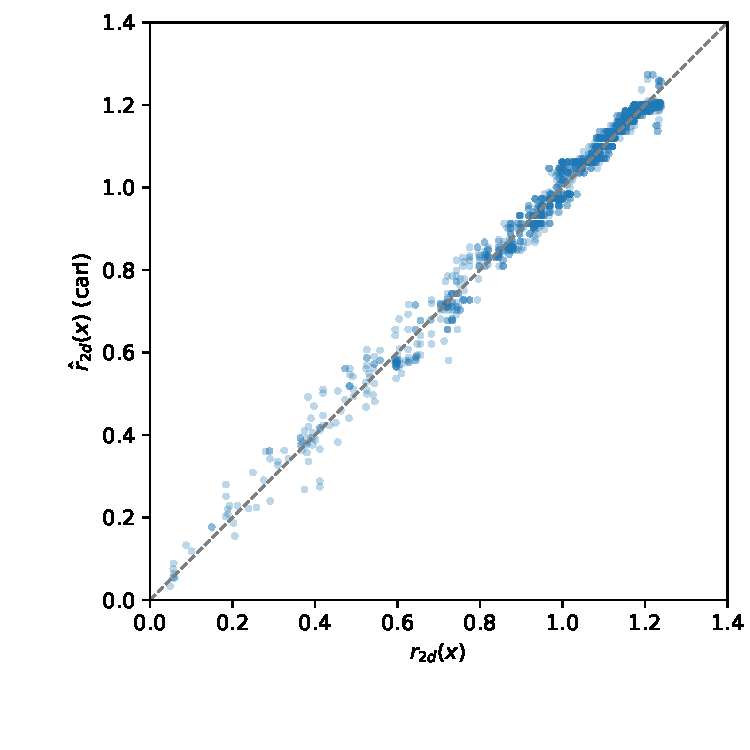
\includegraphics[height=0.45\textwidth]{figures/pointwise_tuning_2d/rhat_vs_r_rf.pdf}%
  \caption{Likelihood ratio estimation with the tuned random forest
    for the 2D case. Left: Distribution of
    \toolfont{carl}'s estimate $\hat{r}(\boldx)$ as a function of the
    observables. Right: scatter plot between the true $r(\boldx)$ and
    the estimate $\hat{r}(\boldx)$}.
  \label{fig:pointwise_tuning_2d_rf_performance}
\end{figure}

\begin{figure}
  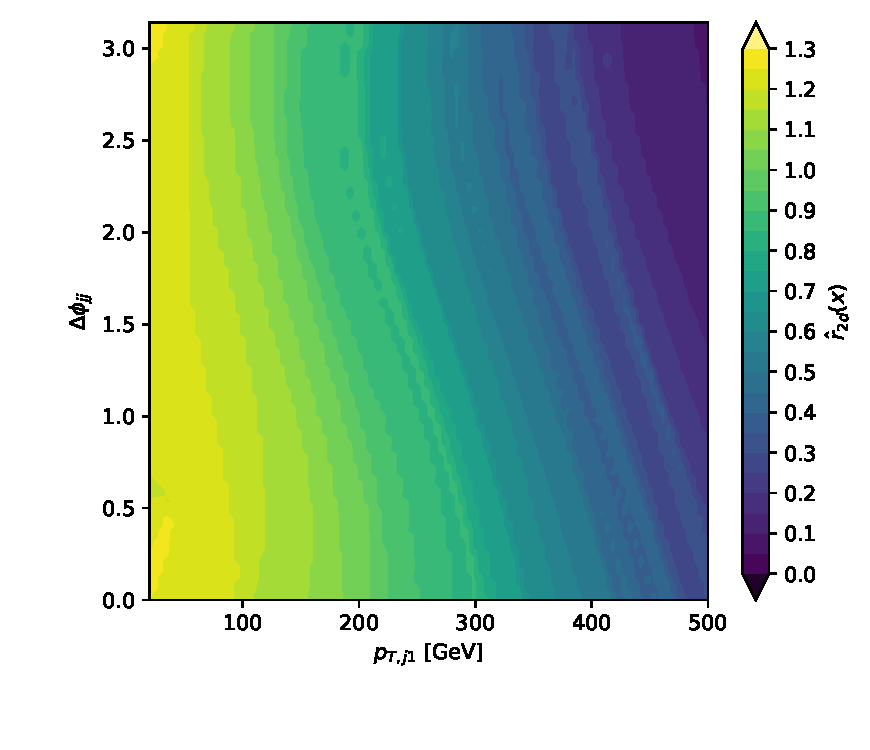
\includegraphics[height=0.45\textwidth]{figures/pointwise_tuning_2d/rhat_over_x_grid_mlp.pdf}
  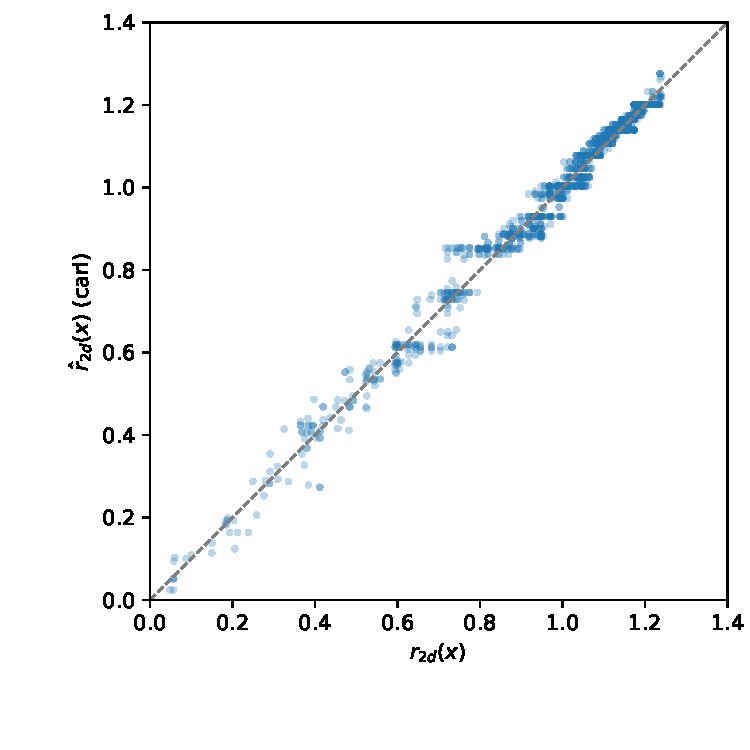
\includegraphics[height=0.45\textwidth]{figures/pointwise_tuning_2d/rhat_vs_r_mlp.pdf}
  \caption{Likelihood ratio estimation with the tuned neural network
    for the 2D case. Left: Distribution of
    \toolfont{carl}'s estimate $\hat{r}(\boldx)$ as a function of the
    observables. Right: scatter plot between the true $r(\boldx)$ and
    the estimate $\hat{r}(\boldx)$}.
  \label{fig:pointwise_tuning_2d_mlp_performance}
\end{figure}

In Figures~\ref{fig:pointwise_tuning_2d_rf_performance} and
\ref{fig:pointwise_tuning_2d_mlp_performance} we show how well
\toolfont{carl} can estimate the true likelihood ratio $r(\boldx)$
with the tuned classifiers given in the right column of
\autoref{tbl:pointwise_tuning_2d_parameters}.

Next, we vary all parameters one by one and see how this affects the
mean squared error of $\log \hat{r}(\boldx)$. The results are shown in
Figures~\ref{fig:pointwise_tuning_2d_rf_tuning} to
\ref{fig:pointwise_tuning_2d_carl_tuning}.

\begin{figure}
  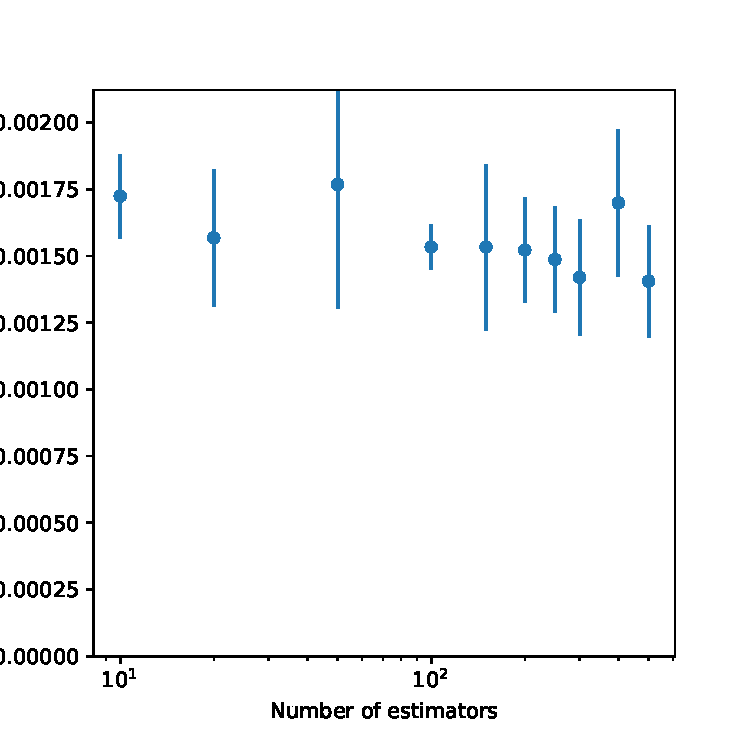
\includegraphics[width=0.45\textwidth]{figures/pointwise_tuning_2d/mse_rf_n_estimators.pdf}%
  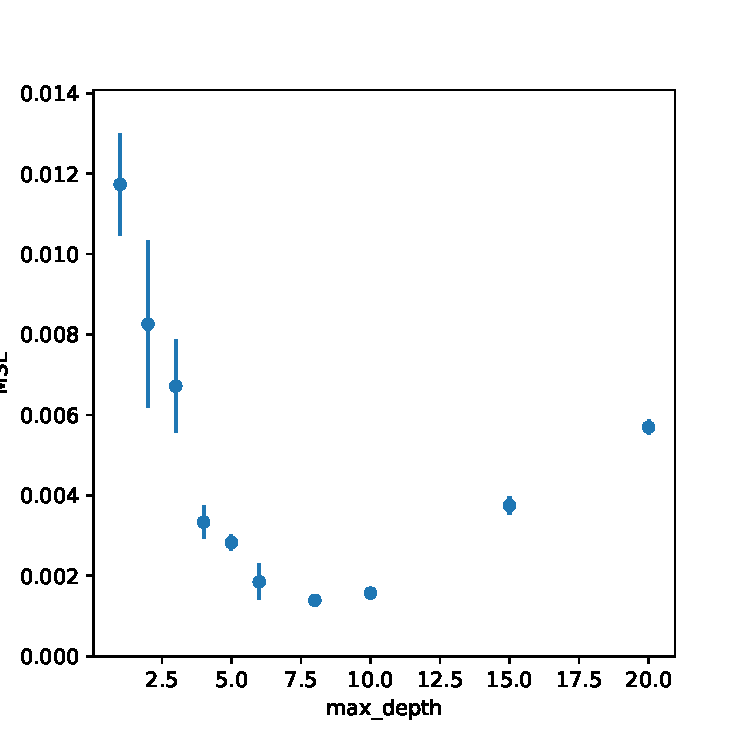
\includegraphics[height=0.45\textwidth]{figures/pointwise_tuning_2d/mse_rf_max_depths.pdf}\\%
  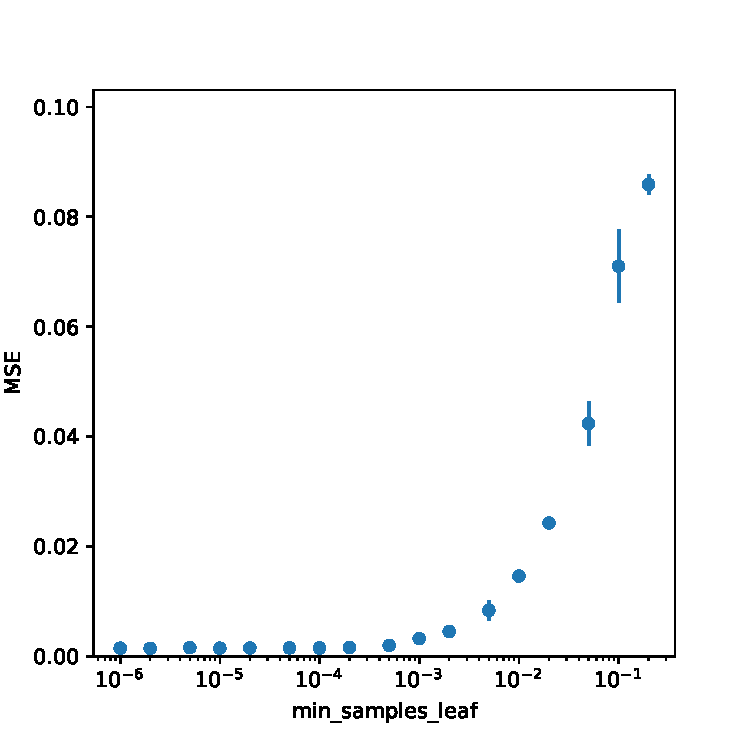
\includegraphics[height=0.45\textwidth]{figures/pointwise_tuning_2d/mse_rf_min_samples_leaf.pdf}%
  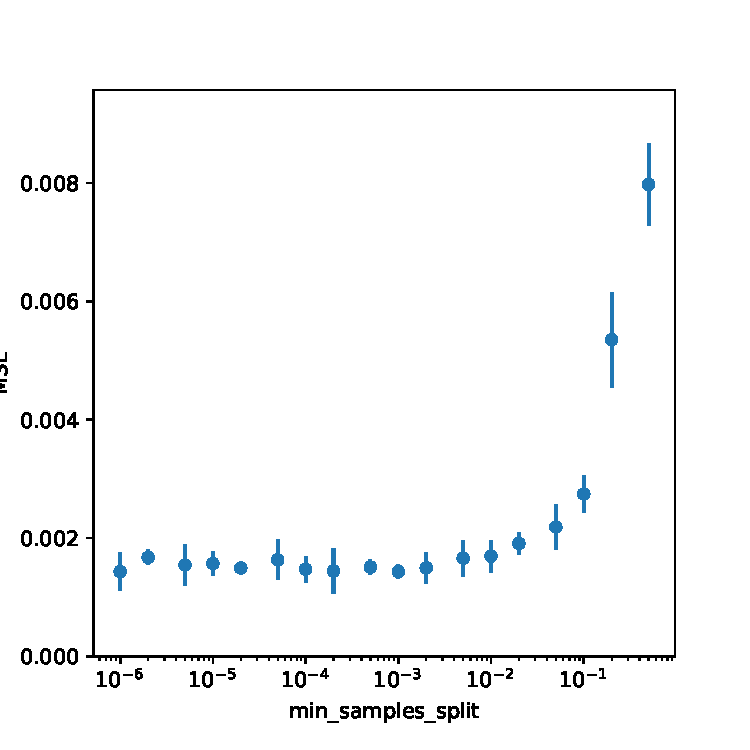
\includegraphics[height=0.45\textwidth]{figures/pointwise_tuning_2d/mse_rf_min_samples_splits.pdf}%
  \caption{carl performance as a function of the random forest
    hyperparameters. We show the mean squred error of the estimated
    log likelihood ratio between two benchmark points for the 2D
    case. Each data point shows the mean of five calculations, the
    error bars are $95\%$ confidence intervals.}
  \label{fig:pointwise_tuning_2d_rf_tuning}
\end{figure}

\begin{figure}
  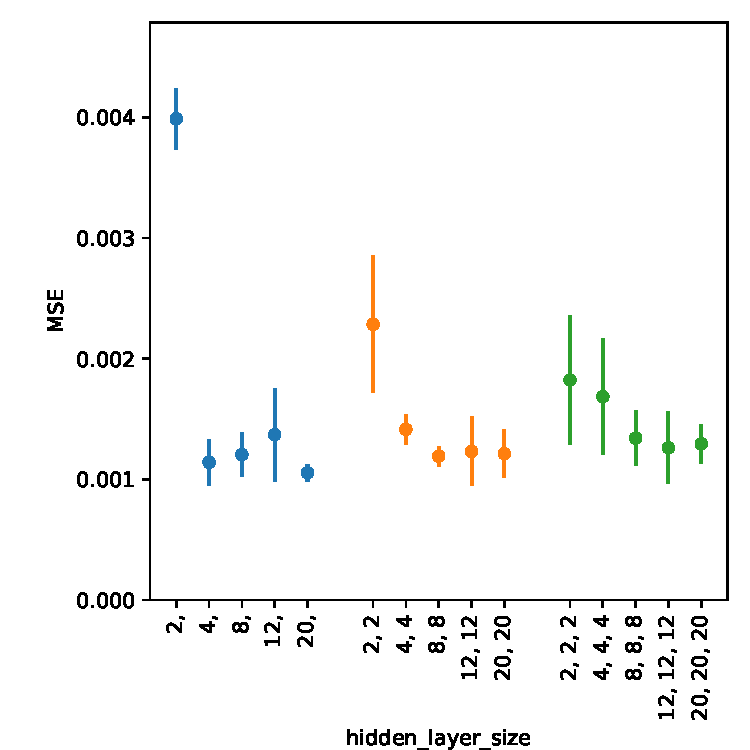
\includegraphics[width=0.45\textwidth]{figures/pointwise_tuning_2d/mse_mlp_hidden_layer_sizes.pdf}%
  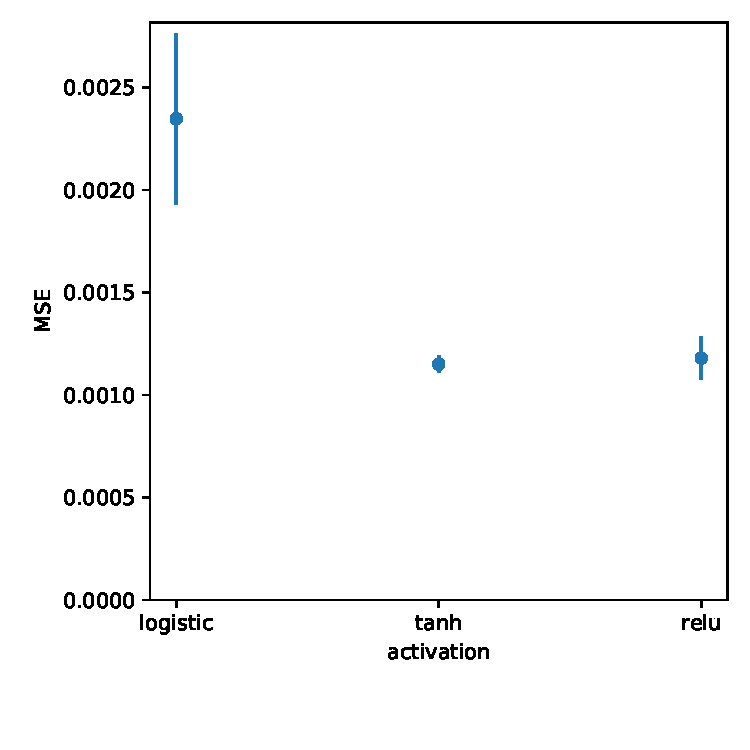
\includegraphics[height=0.45\textwidth]{figures/pointwise_tuning_2d/mse_mlp_activation.pdf}\\%
  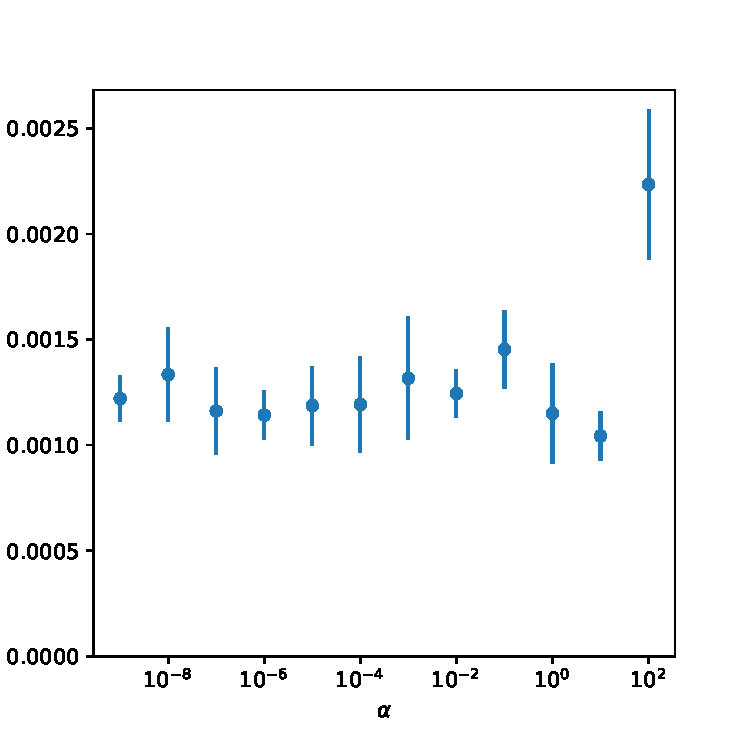
\includegraphics[height=0.45\textwidth]{figures/pointwise_tuning_2d/mse_mlp_alpha.pdf}%
  \caption{carl performance as a function of the neural network
    hyperparameters. Mean squred error of the estimated log likelihood
    ratio between two benchmark points for the 2D case. Each data
    point shows the mean of five calculations, the error bars are
    $95\%$ confidence intervals.}
  \label{fig:pointwise_tuning_2d_mlp_tuning}
\end{figure}

The parameters that are best for the classification problem also work
best for the estimation of the likelihood ratio with
$\toolfont{carl}$. The performance of the random forest crucially
depends on the maximal depth, while the neural network works well with
pretty much any setup, as long as each layer has enough neurons. To
reduce training time, we therefore define a final setup of the neural
network with a reduced number of 8 neurons in each hidden layer. For
the random forest, we stick to the parameters in the right column of
\autoref{tbl:pointwise_tuning_2d_parameters}.

\begin{figure}
  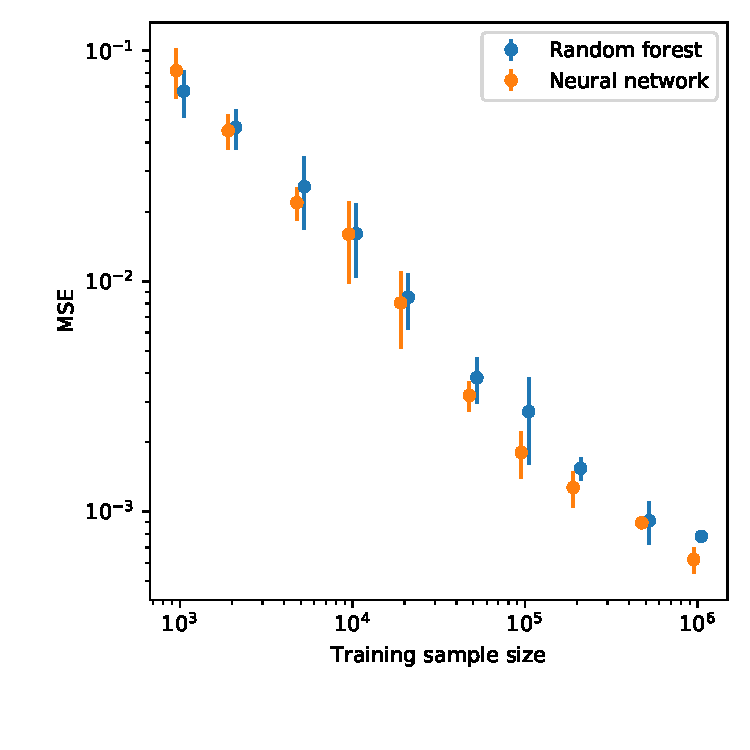
\includegraphics[width=0.45\textwidth]{figures/pointwise_tuning_2d/mse_training_sample_size.pdf}%
  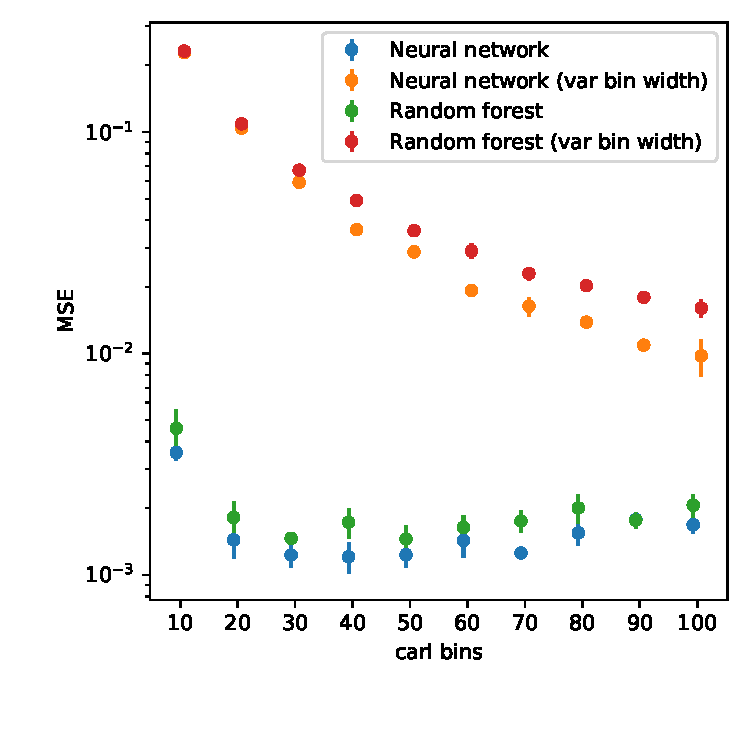
\includegraphics[height=0.45\textwidth]{figures/pointwise_tuning_2d/mse_carl_bins.pdf}%
  \caption{carl performance as a function of the training sample size
    (left) and the number of bins in the \toolfont{carl} calibration
    histograms.  We show the mean squred error of the estimated log
    likelihood ratio between two benchmark points for the 2D
    case. Each data point shows the mean of five calculations, the
    error bars are $95\%$ confidence intervals.}
  \label{fig:pointwise_tuning_2d_carl_tuning}
\end{figure}

\autoref{fig:pointwise_tuning_2d_carl_tuning} shows the effect of the
size of the training samples as well as the binning of
\toolfont{carl}'s calibration histograms.  Regardless of the
problematic distribution of weights in the input samples (see
\autoref{fig:sample_weights}), the performance becomes much better
with larger training samples. We pick a size of 200\,000 events as a
balance between computation time and performance. The calibration
histograms should have at least 20 bins, and variable bin widths do
not seem to work well at all.

\begin{figure}
  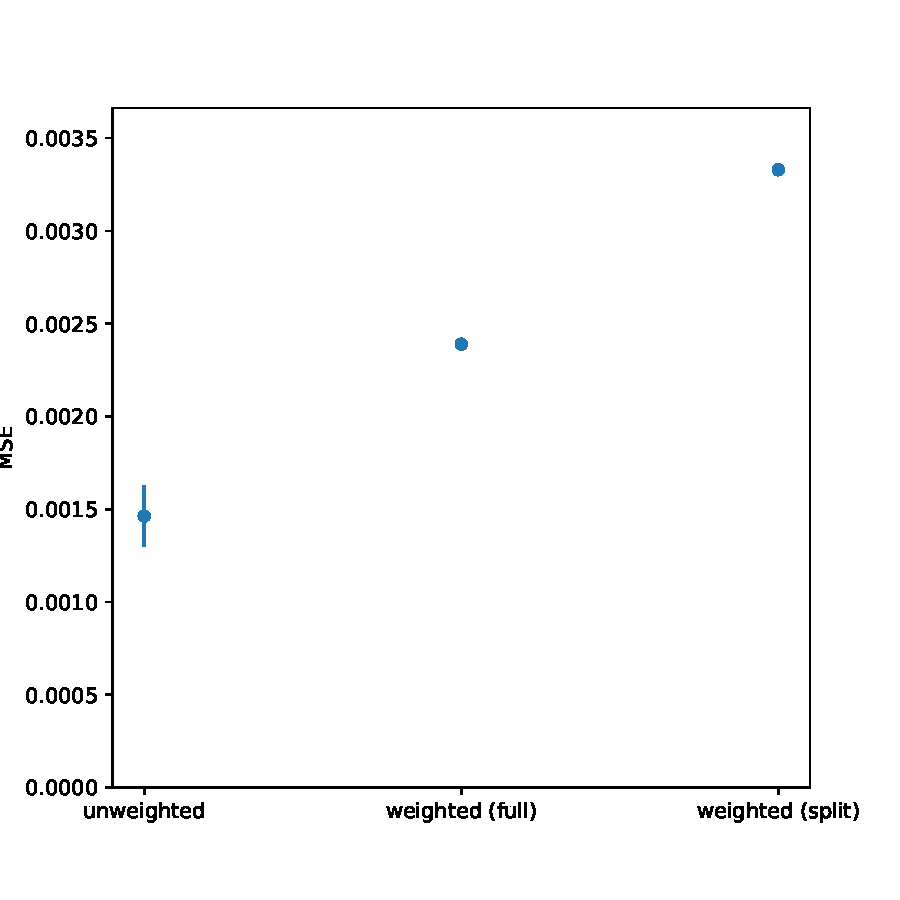
\includegraphics[height=0.45\textwidth]{figures/pointwise_tuning_2d/mse_weighted_events.pdf}%
  \caption{carl performance with weighted training samples. We show
    the mean squred error of the estimated log likelihood ratio between
    two benchmark points based on the two-dimensional feature
    space.}
  \label{fig:pointwise_tuning_2d_weighted}
\end{figure}

As demonstrated in \autoref{fig:pointwise_tuning_2d_weighted},
training random forests with weighted samples does not improve the
performance, even if the full training sample of 5 million events is
used. However, we did not try to tune the random forest parameters
with weighted input.

\begin{figure}
  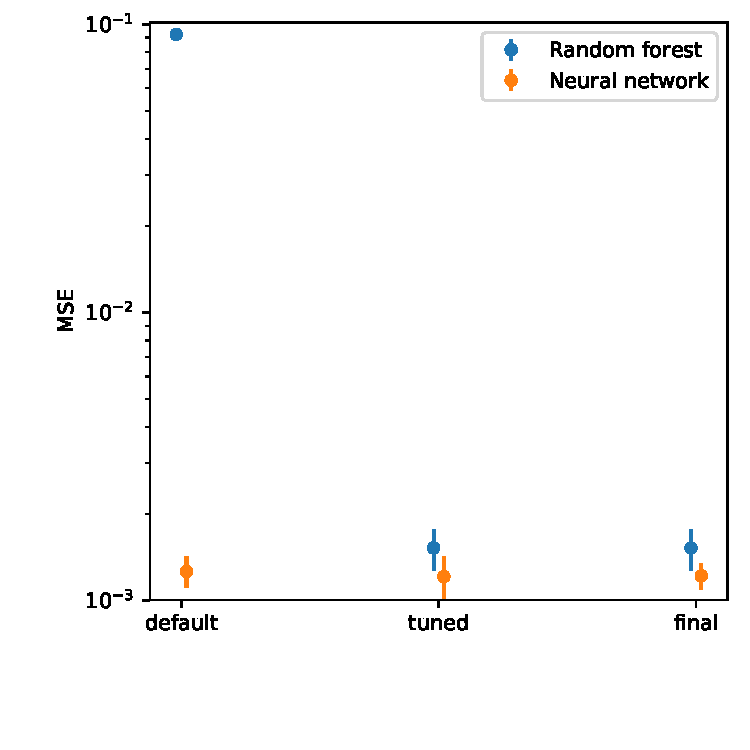
\includegraphics[height=0.45\textwidth]{figures/pointwise_tuning_2d/mse_final.pdf}%
  \caption{carl performance for the 2D case with \toolfont{sklearn}
    default hyperparameters, the best parameters according to the
    initial hyperparameter scan, and the final parameters as defined
    in the text. We show the mean squred error of the estimated log
    likelihood ratio between two benchmark points. Each data point
    shows the mean of five calculations, the error bars are $95\%$
    confidence intervals.}
  \label{fig:pointwise_tuning_2d_final}
\end{figure}

We summarise \toolfont{carl}'s performance before and after tuning and
compare the two classifiers in
\autoref{fig:pointwise_tuning_2d_final}. We find that the neural
network performs slightly better, and is much less dependent on the
choice of parameters. The output of \toolfont{carl} with this final
neural network setup is shown in
\autoref{fig:pointwise_tuning_2d_final_performance}. As a matter of
fact, the smooth neural net output might be closer to the real
likelihood ratio than our calculated $r(\boldx)$ with its binning
artefacts.

\begin{figure}
  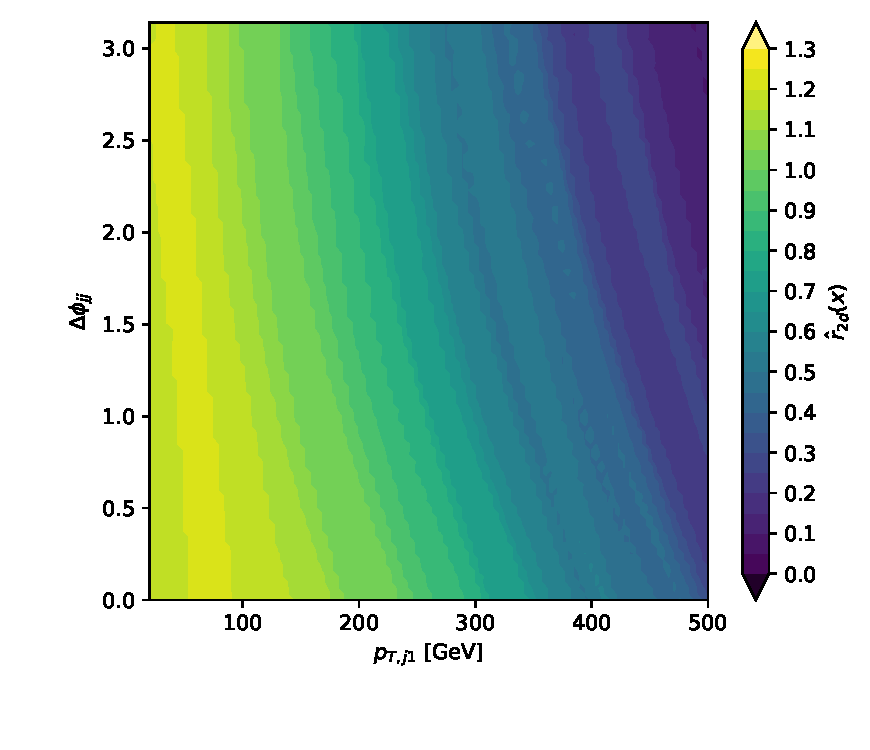
\includegraphics[height=0.45\textwidth]{figures/pointwise_tuning_2d/rhat_over_x_grid_final.pdf}
  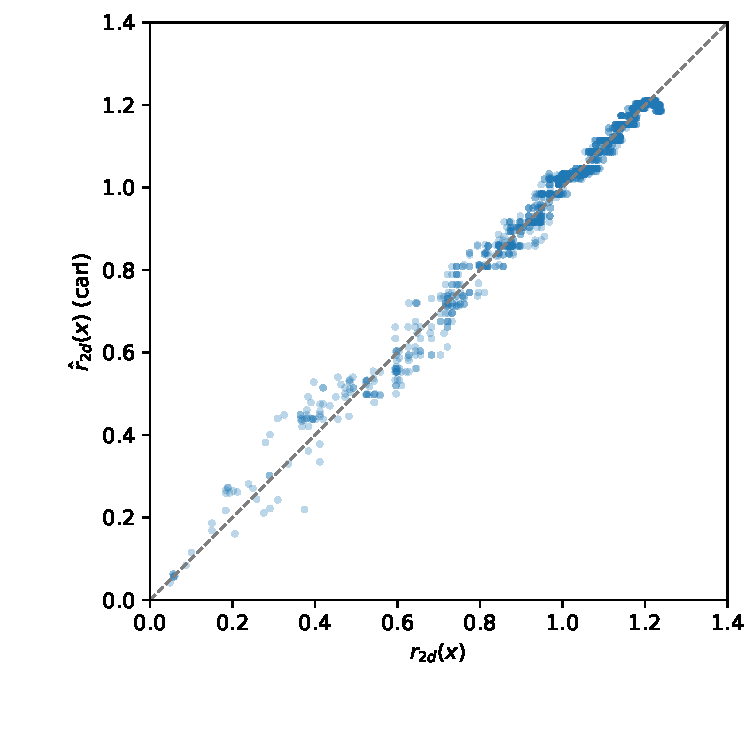
\includegraphics[height=0.45\textwidth]{figures/pointwise_tuning_2d/rhat_vs_r_final.pdf}
  \caption{Likelihood ratio estimation with the final neural network
    for the 2D case. Left: Distribution of \toolfont{carl}'s estimate
    $\hat{r}(\boldx)$ as a function of the observables. Right: scatter
    plot between the true $r(\boldx)$ and the estimate
    $\hat{r}(\boldx)$}.
  \label{fig:pointwise_tuning_2d_final_performance}
\end{figure}






%%%%%%%%%%%%%%%%%%%%%%%%%%%%%%%%%%%%%%%%%%%%%%%%%%%%%%%%%%%%
\subsubsection{Validation}
%%%%%%%%%%%%%%%%%%%%%%%%%%%%%%%%%%%%%%%%%%%%%%%%%%%%%%%%%%%%

After tuning the parameters for one specific choice of benchmark
points, we now check how well these settings work for the likelihood ratio
between two different benchmark points
%
\begin{equation}
  \boldtheta_0' = \twovec{0.5} {-0.5} \,, \quad
  \boldtheta_1' = \twovec{-0.5} {0.5} \,.
  \label{eq:pointwise_validation_benchmarks}
\end{equation}

\begin{figure}
  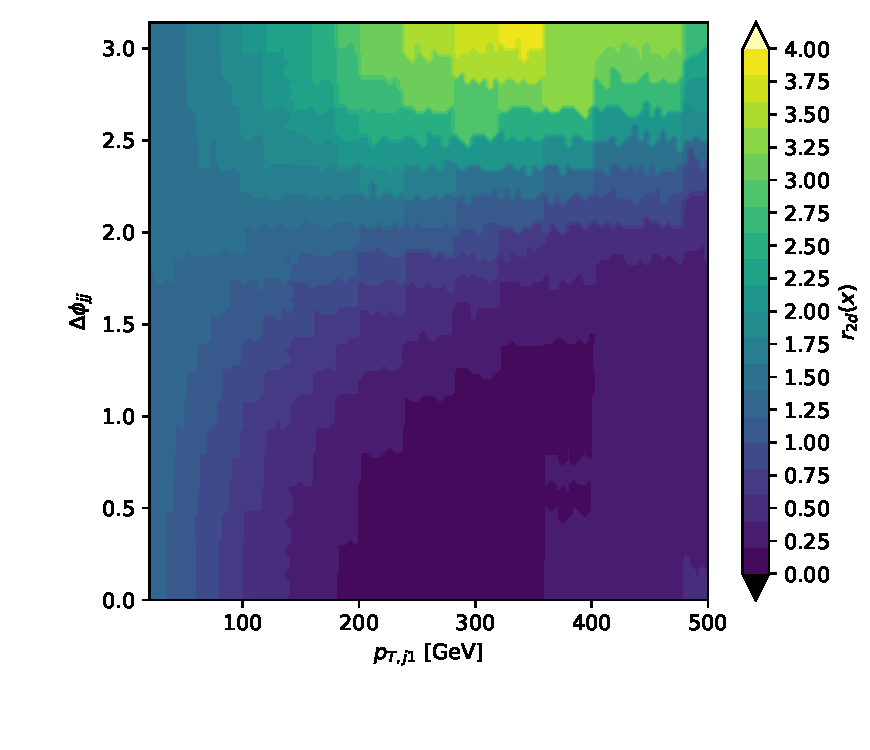
\includegraphics[height=0.45\textwidth]{figures/pointwise_tuning_2d/r_over_x_grid_alt.pdf}
  \caption{Truth likelihood ratio $r(\boldx)$ between the validation
    benchmark points for the 2D case as a function of the
    observables.}
  \label{fig:pointwise_validation_2d_r_x}
\end{figure}

\autoref{fig:pointwise_validation_2d_r_x} shows the truth likelihood
ratio between the validation benchmark points of
\autoref{eq:pointwise_validation_benchmarks} as a function of the two
observables.

\begin{figure}
  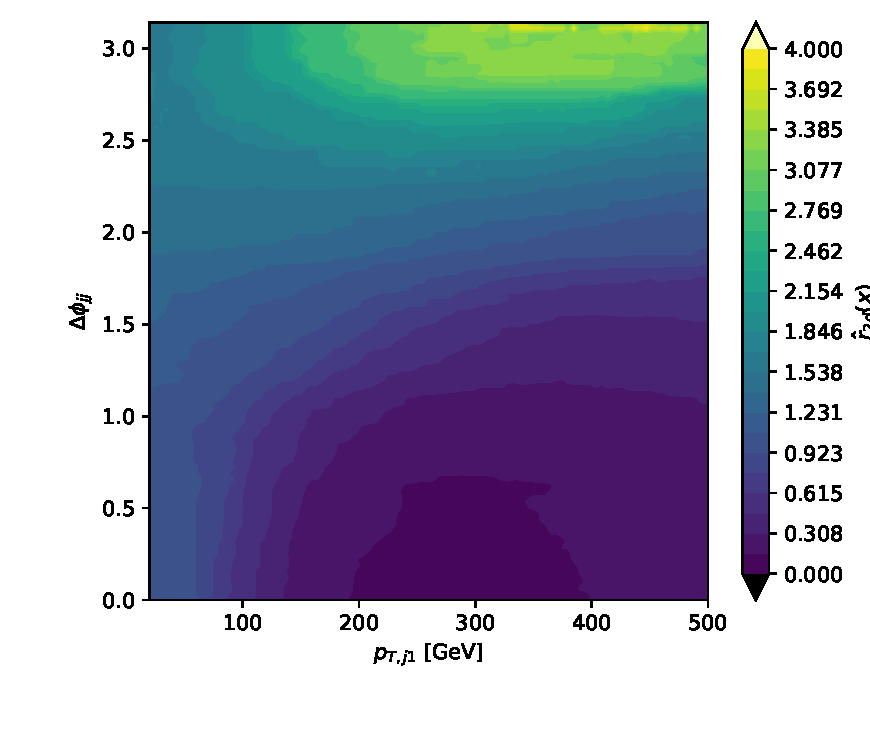
\includegraphics[height=0.45\textwidth]{figures/pointwise_tuning_2d/rhat_over_x_grid_rf_alt.pdf}%
  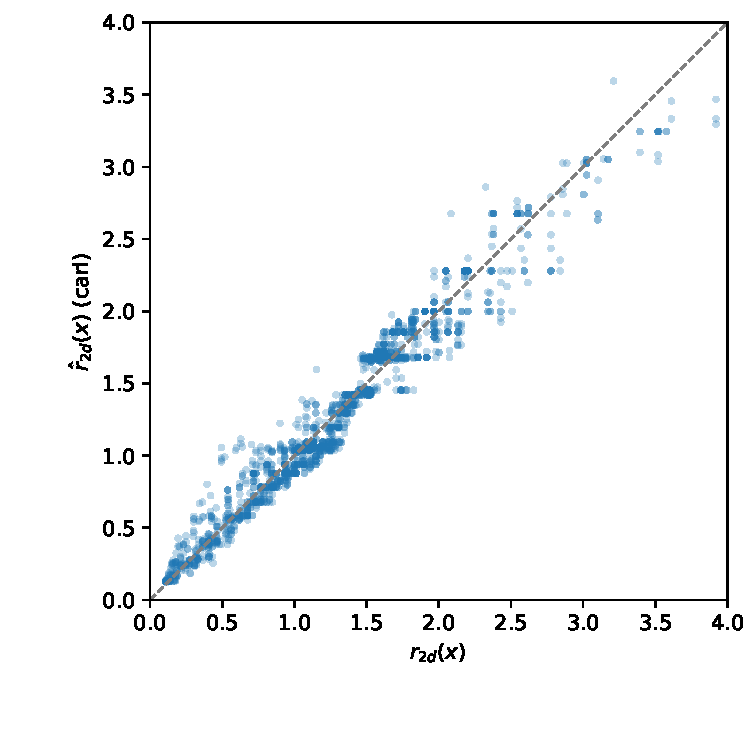
\includegraphics[height=0.45\textwidth]{figures/pointwise_tuning_2d/rhat_vs_r_rf_alt.pdf}%
  \caption{Likelihood ratio estimation with the tuned random forest on
    separate validation hypotheses for the 2D case. Left: Distribution
    of \toolfont{carl}'s estimate $\hat{r}(\boldx)$ as a function of
    the observables. Right: scatter plot between the true $r(\boldx)$
    and the estimate $\hat{r}(\boldx)$}.
  \label{fig:pointwise_validation_2d_rf_performance}
\end{figure}

\begin{figure}
  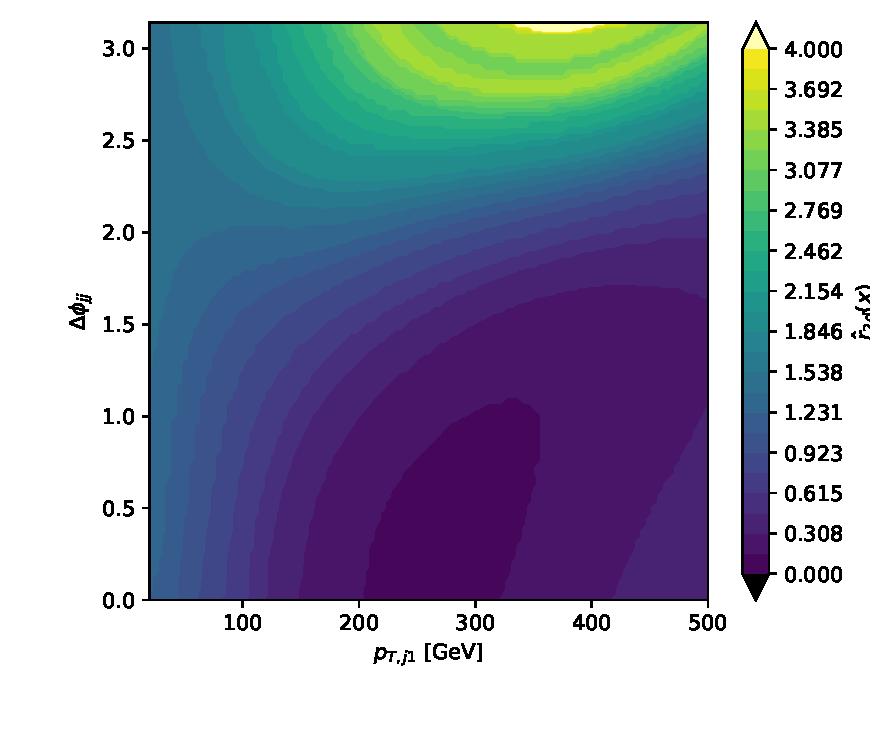
\includegraphics[height=0.45\textwidth]{figures/pointwise_tuning_2d/rhat_over_x_grid_final_alt.pdf}
  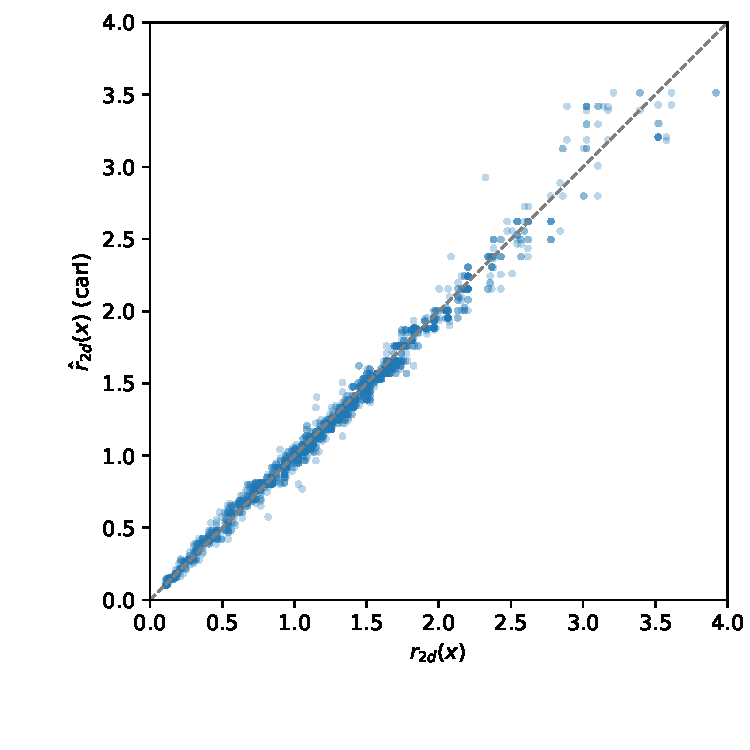
\includegraphics[height=0.45\textwidth]{figures/pointwise_tuning_2d/rhat_vs_r_final_alt.pdf}
  \caption{Likelihood ratio estimation with the neural network on
    separate validation hypotheses for the 2D case.  Left:
    Distribution of \toolfont{carl}'s estimate $\hat{r}(\boldx)$ as a
    function of the observables. Right: scatter plot between the true
    $r(\boldx)$ and the estimate $\hat{r}(\boldx)$}.
  \label{fig:pointwise_validation_2d_mlp_performance}
\end{figure}

\begin{figure}
  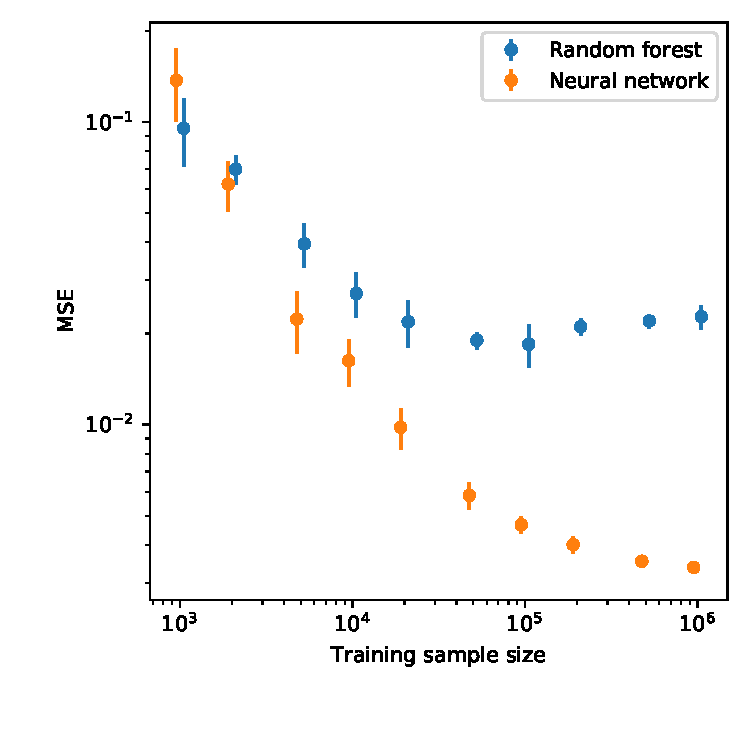
\includegraphics[height=0.45\textwidth]{figures/pointwise_tuning_2d/mse_training_sample_size_alt.pdf}
  %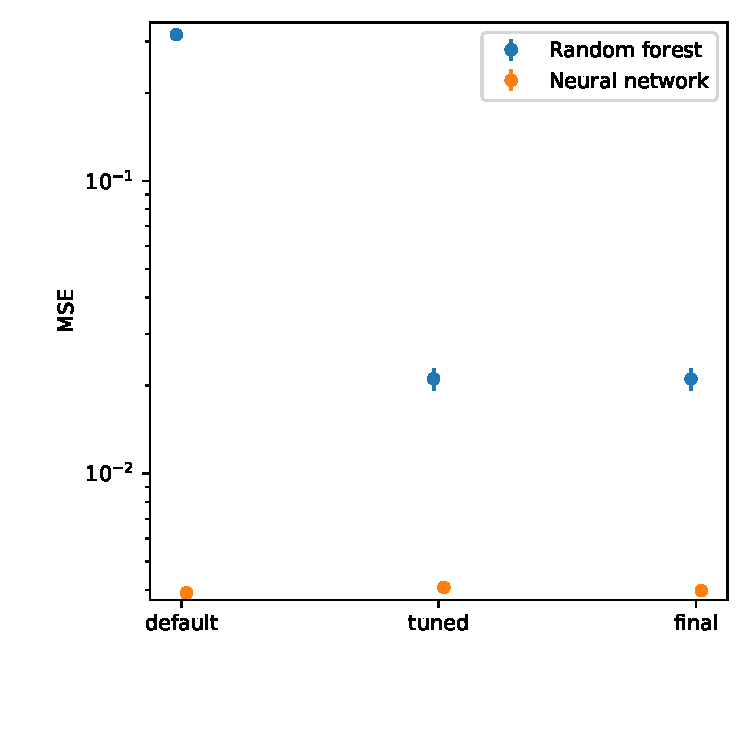
\includegraphics[height=0.45\textwidth]{figures/pointwise_tuning_2d/mse_final_alt.pdf}
  \caption{carl performance on the validation hypotheses for different
    training sample sizes and classifiers).  We show the mean squred
    error of the estimated log likelihood ratio between two validation
    benchmark points for the 2D case. Each data point shows the mean
    of five calculations, the error bars are $95\%$ confidence
    intervals.}
  \label{fig:pointwise_validation_2d_overview}
\end{figure}

In Figures~\ref{fig:pointwise_validation_2d_rf_performance} to
\ref{fig:pointwise_validation_2d_overview} we show
\toolfont{carl}'s estimation based on the final settings tuned in
\autoref{sec:pointwise_tuning_2d}. How this performance depends on the
choice of hyperparameters is illustrated in
\autoref{fig:pointwise_validation_2d_tuning}.

\begin{figure}
  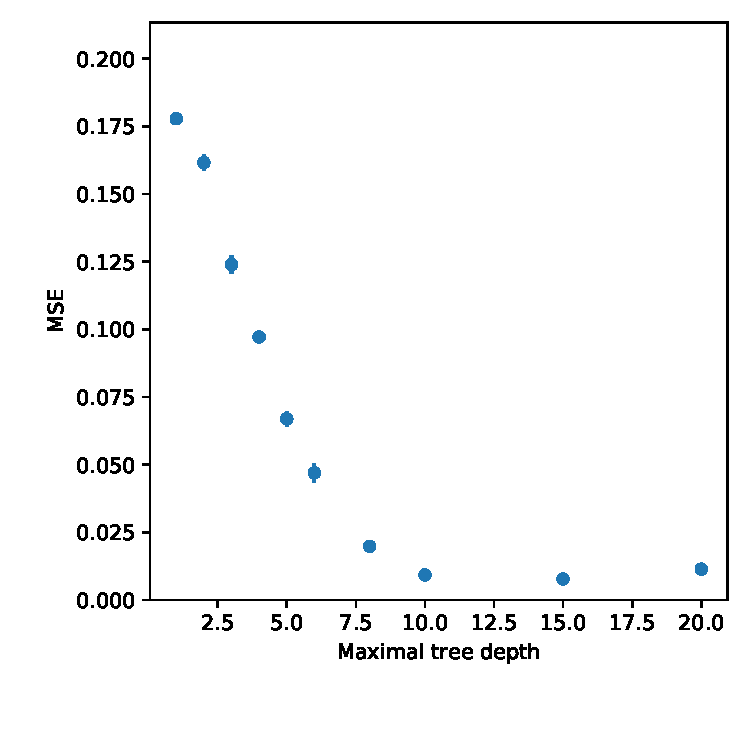
\includegraphics[height=0.45\textwidth]{figures/pointwise_tuning_2d/mse_rf_max_depths_alt.pdf}%
  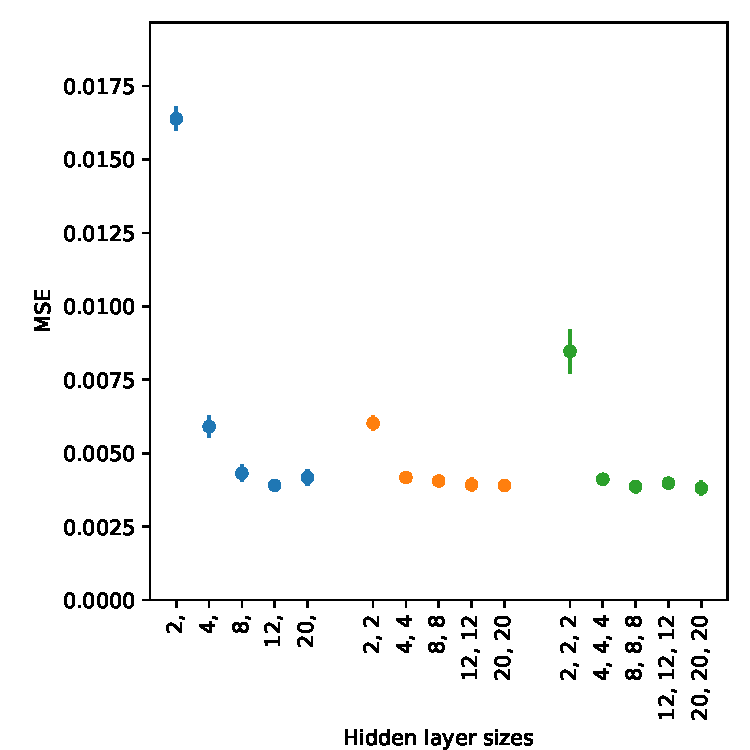
\includegraphics[width=0.45\textwidth]{figures/pointwise_tuning_2d/mse_mlp_hidden_layer_sizes_alt.pdf}%
  \caption{carl performance on the validation hypotheses for different
    hyperparameters.  We show the mean squred error of the estimated
    log likelihood ratio between two validation benchmark points for
    the 2D case. Each data point shows the mean of five calculations,
    the error bars are $95\%$ confidence intervals.}
  \label{fig:pointwise_validation_2d_tuning}
\end{figure}

All in all, we find that the neural net performs very well without
further fine-tuning, \ie that the same settings optimised on the
comparison of $\boldtheta_0$ versus $\boldtheta_1$ also work well for
$\boldtheta_0'$ versus $\boldtheta_1'$. The random forest, on the
other hand, is not so flexible. The two different hypothesis
comparisons require different choices of the maximal depth of the
trees, and what works best for one choice of parameter points leads to
a poor performance for a different choice. 



%%%%%%%%%%%%%%%%%%%%%%%%%%%%%%%%%%%%%%%%%%%%%%%%%%%%%%%%%%%%
\subsubsection{Likelihood contours}
%%%%%%%%%%%%%%%%%%%%%%%%%%%%%%%%%%%%%%%%%%%%%%%%%%%%%%%%%%%%

After optimizing our classifier setup on the distinction between two
distinct hypotheses, and validating the results on another two
hypotheses, we now turn towards the more relevant problem of
estimating $\boldtheta$ based on some measurements. We generate
25\,000 toy events sampled from the probability distribution for the
SM,
%
\begin{equation}
  \boldtheta_{\text{observed}} = \twovec 0 0 \,.
\end{equation} 
%
For 100 points randomly sampled in $\boldtheta \in [-0.9,0.9]^2$, we
calculate the true expected likelihood ratio to
%
\begin{equation}
  \boldtheta_{1} = \twovec {-0.23} {0.30}
\end{equation}
%
as well as the corresponding \toolfont{carl} estimate. Finally, we
interpolate between these points with a Gaussian Process with Mat\'ern
kernel with $\nu = 0.5$.

Following the results of the previous sections, for the
two-dimensional feature space we use a neural network with two hidden
layers of 8 neurons each, a $\tanh$ activation function, and a
regulator $\alpha = 0.001$. The training samples consist of 200\,000
unweighted samples each, and the $\toolfont{carl}$ default for the
fixed-size binning of the calibration histograms is used.

\begin{figure}
  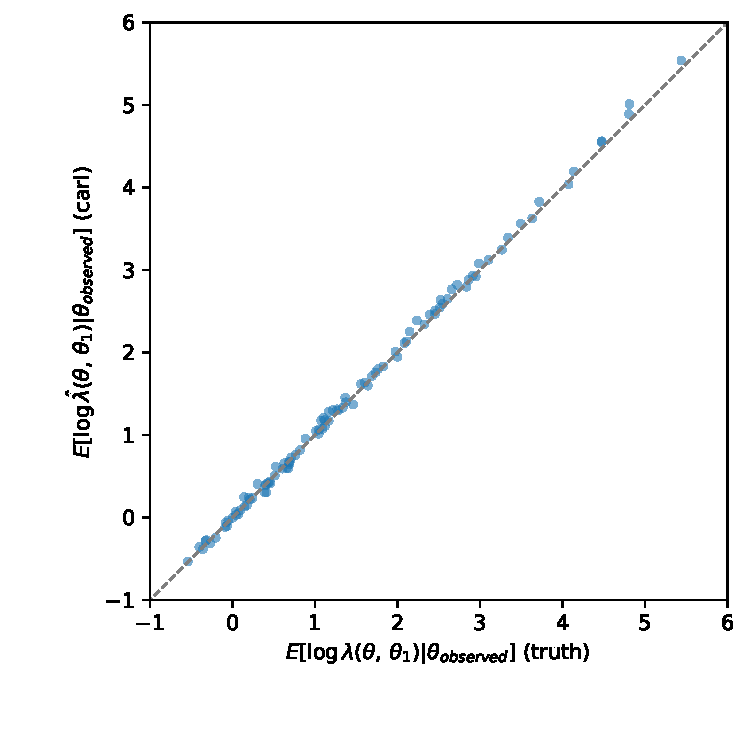
\includegraphics[height=0.45\textwidth]{figures/pointwise_inference/llr_truth_vs_carl_2d.pdf}%
  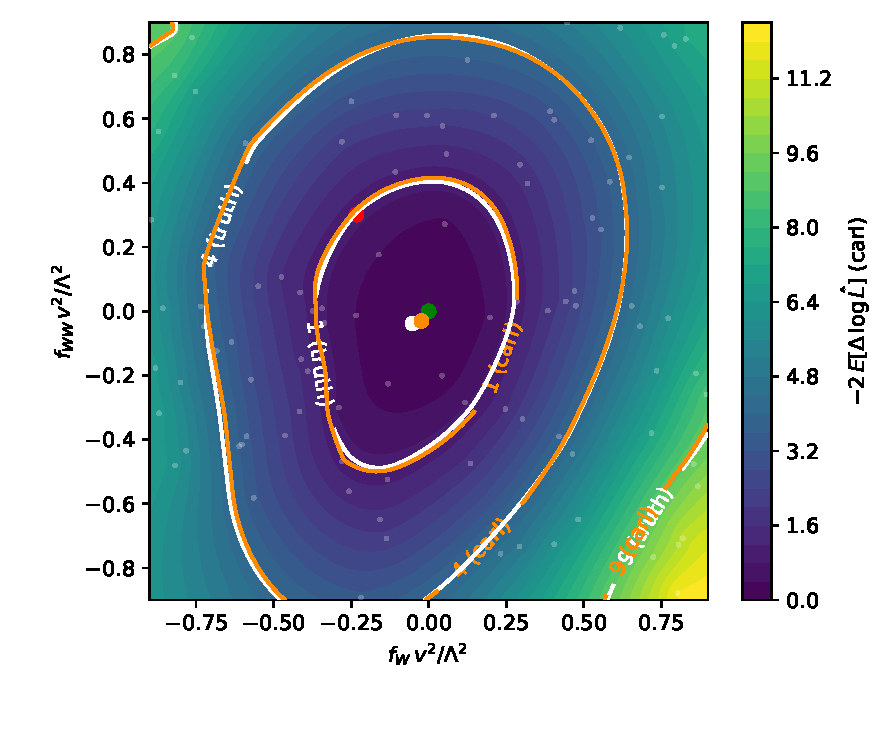
\includegraphics[height=0.45\textwidth]{figures/pointwise_inference/llr_gp_carl_2d.pdf}%
  \caption{Inference from truth likelihood ratio and \toolfont{carl}'s
    estimate for the 2D case. Left: scatter plot showing the
    difference between the exact expected likelihood ratio for 100
    randomly sampled points and $\boldtheta_1$ and \toolfont{carl}'s
    estimate. Right: true (white) and approximate (orange) likelihood
    contours, using a Gaussian Process for interpolation. The white
    and orange dots show the exact and approximate maximum-likelihood
    estimators. The green and red dots show
    $\boldtheta_{\text{observed}}$ and $\boldtheta_1$,
    respectively. Finally, the small grey dots show the sampled
    parameter points at which the likelihood ratio was evaluated.}
  \label{fig:pointwise_inference_2d}
\end{figure}

In \autoref{fig:pointwise_inference_2d} we show the results for the
two-dimensional feature space. The approximate likelihood map agrees
impressively well with the exact one. 







%%%%%%%%%%%%%%%%%%%%%%%%%%%%%%%%%%%%%%%%%%%%%%%%%%%%%%%%%%%%
\subsection{ROC curves}
\label{sec:appendix_ROC}
%%%%%%%%%%%%%%%%%%%%%%%%%%%%%%%%%%%%%%%%%%%%%%%%%%%%%%%%%%%%


\begin{figure}
  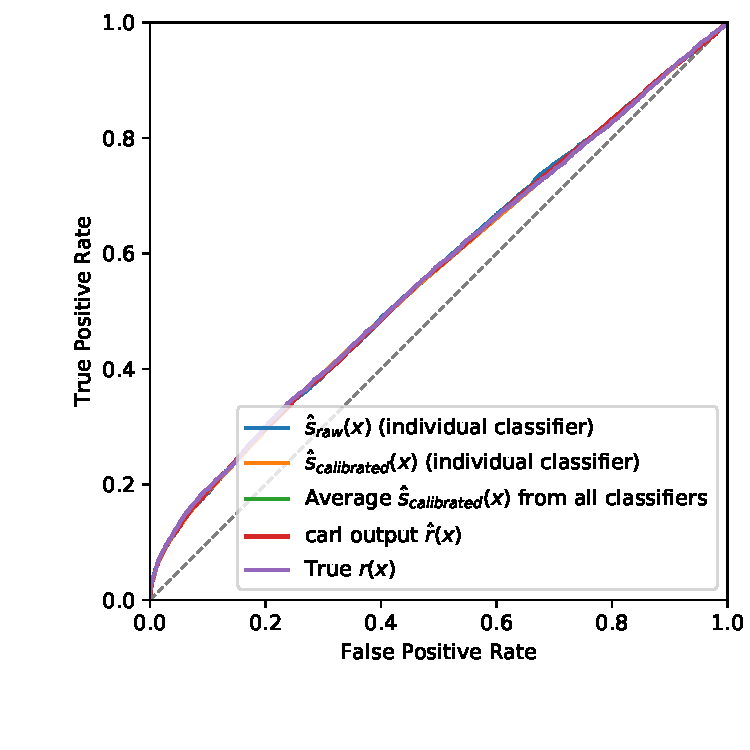
\includegraphics[height=0.45\textwidth]{figures/pointwise_tuning_full/roc_smart_rf.pdf}
  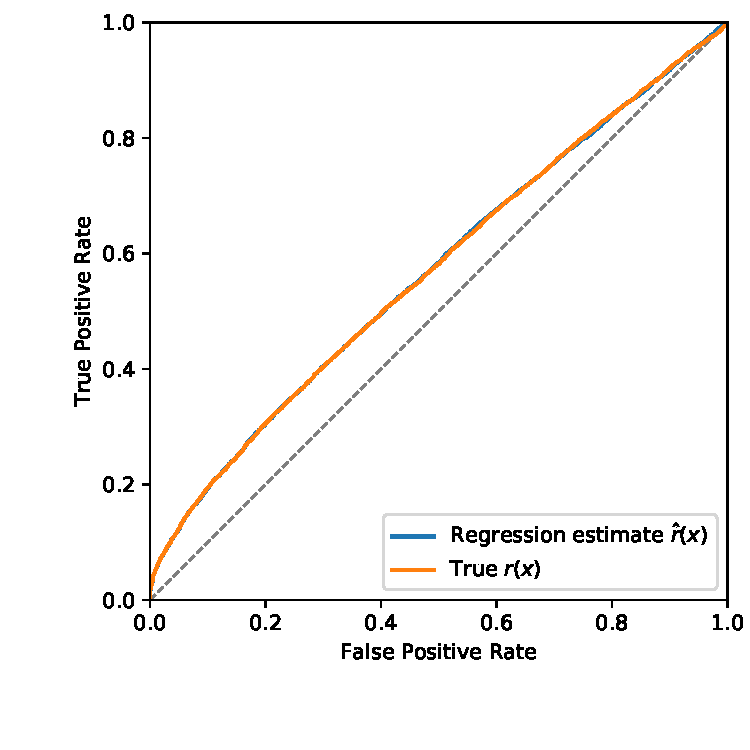
\includegraphics[height=0.45\textwidth]{figures/pointwise_regression_tuning_full/roc_smart_mlp_logr.pdf}
  \caption{ROC curves for the classification between event samples
    based on $\boldtheta_0$ and $\boldtheta_1$ as defined in
    \autoref{eq:pointwise_tuning_benchmarks}. Left: calibrated
    classifiers (with random forests as described in
    \autoref{sec:pointwise_tuning_full}). Right: regression (with a
    neural network as described in
    \autoref{sec:pointwise_regression_tuning}.}
  \label{fig:pointwise_tuning_roc}
\end{figure}

In Figure~\ref{fig:pointwise_tuning_roc} we show some ROC curves
corresponding to the classification problem of
\autoref{sec:pointwise_tuning_full}. We compare the TPRs and FPRs of
six different scores:
%
\begin{itemize}
  \item the raw output $\hat{s}(\boldx)$ of one random forest, using the medium feature set as input and the tuned settings described in \autoref{sec:pointwise_tuning_full};
  \item the same output, calibrated with the histogram method;
  \item the average of the outputs of five such calibrated random forests;
  \item the corresponding $\toolfont{carl}$ estimate $\hat{r}(\boldx)$;
  \item the estimate $\hat{r}(\boldx)$ based on a regressor as described in \autoref{sec:pointwise_regression_tuning}; and
  \item the true $r(\boldx)$, which defines the optimal classifier according to the Neyman-Pearson lemma.
\end{itemize}
%
The resulting ROC curves are pretty much indistinguishable. This shows
that the classification problem between two hypotheses is solved
nearly optimally by our learning setup, and that this is much easier
than the regression\,/\,density estimation problem of learning
$r(\boldx)$.